\chapter{Applications des méthodes de descente au deep learning}
\section{Introduction et Motivation}
L'intelligence artificielle représente un ensemble de théories et techniques dont le but est de simuler l'intelligence chez la machine. C'est un concept datant des années 1950 mais qui revient à la mode depuis le début du XXIe siècle, à la fois grâce à des avancées technologiques nombreuses mais également dans les mentalités par le biais de films de science fiction. On peut notamment citer la trilogie Matrix, décrivant un monde dystopique où les machines dominent les hommes après avoir dépassé un stade d'intelligence inattendu. Cependant malgré le fait que l'intelligence artificielle a beaucoup évolué ces dernières années, nous sommes encore loin de ce résultat. Actuellement, les appareils que nous utilisons sont généralement limités à un domaine, par exemple la traduction, la navigation... car les systèmes dit intelligents doivent passer par une phase d'apprentissage. Mais cela pourrait bien changer avec le développement du deep learning ou apprentissage profond.

\subsection{Intelligence artificielle, machine learning et deep learning}
	Mais qu'est-ce que l'apprentissage profond ? C'est en fait un sous-domaine du machine learning, lui même étant une branche de l'intelligence artificielle. Voici une représentation sous forme d'arbres permettant de visualiser différentes approches de l'IA : 
	\begin{figure}[H]
		\centering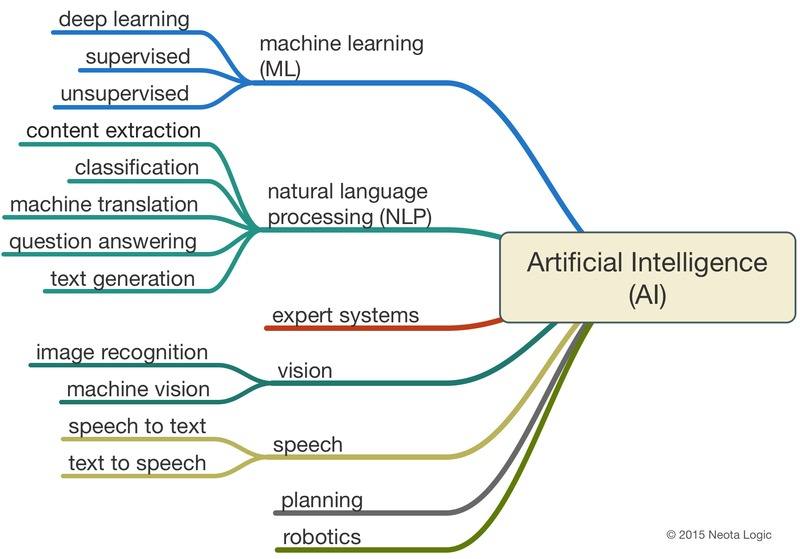
\includegraphics[width=0.7\linewidth]{images/branches}
		\caption{Approches de l'IA}
	\end{figure}
	Pour mieux comprendre ce que sont machine learning et deep learning commençons par les \textit{systèmes experts}. Ce sont des logiciels très spécialisés dont le but est de reproduire la "pensée" d'un expert dans un domaine. Cela permet de remplacer une personne pour une tâche bien précise. Par exemple, le premier système expert mis au point, Dendral (en 1965) permettait d'identifier les consitituants chimiques d'un matériau. Les systèmes experts reposent sur des algorithmes "simples", constitués de conditions "if... then...", pouvant être assimilés à des arbres de décisions. Ils sont donc utilisables uniquement pour des tâches précises et déterminées à l'avance et ne peuvent sortir de leurs bornes d'application. L'apprentissage de la machine est manuelle, c'est l'homme qui doit implémenter toutes les possibilités lui-même.\\
	
	Le machine learning apporte une solution à cela. Dorénavant, l'ordinateur apprend par lui-même. L'homme lui apprend à reconnaitre et à reproduire. On dit qu'on "entraine" la machine. Il faut pour cela lui fournir de grands jeux de données, c'est là qu'intevient le domaine du big data et c'est une des raisons pour lesquelles le développement du machine learning s'est accéléré ces dernières années. Grâce aux données d'entraînement, le programme constitue des données statistiques sur lesquelles il s'appuie ensuite pour faire ses prévisions. \\
	
	Enfin, le deep learning est constitué d'algorithmes permettant au logiciel de s'entrainer lui même. Cette dernière approche est basée sur ce que l'on appelle des "réseaux de neurones" à multiples couches, imitant (plus ou moins) le fonctionnement du cerveau humain. Plus ils reçoivent de données, plus ces réseaux de neurones sont performants.
	
\section{Architecture d'un réseau de neurones}

	\begin{figure}[H]
		\centering
		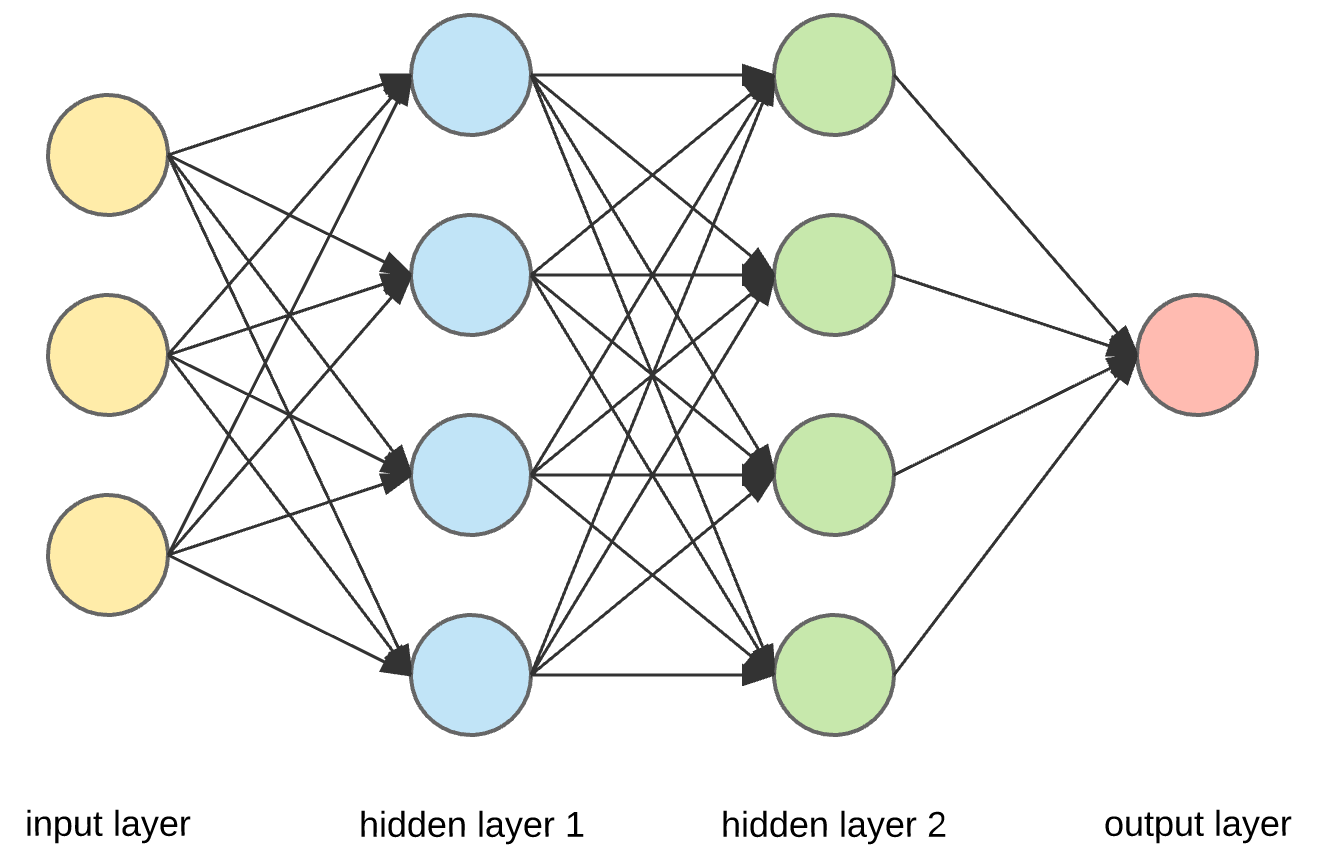
\includegraphics[width=0.75\linewidth]{images/reseau}
		\caption{Architecture d'un réseau de neurones}
	\end{figure}

	Les réseaux de neurones sont formés de plusieurs couches successives, comme on peut le voir sur l'image ci-dessus. Sur ce schéma, les n\oe uds représentent les neurones tandis que les fléches illustrent les "poids". La première couche (en jaune) est la couche d'entrée, elle contient les informations à "traiter". Tout au bout de la chaîne on a une couche de sortie, elle est ici composée d'un seul neurone mais il peut y en avoir plusieurs. Entre les entrées et sorties, on trouve des couches dites "cachées". C'est là que se font tous les calculs. Le réseau de neurone est parcouru dans les deux sens : d'abord de la couche "entrée" à la couche "sortie" (phase de prédiction), puis dans le sens opposé (phase d'apprentissage ou \textit{backpropagation}). Lors de la première phase avant, les valeurs d'entrée sont généralement initialisée de manière aléatoire, puis les valeurs des neurones des couches suivantes sont calculées comme détaillé plus loin. Zoomons donc sur un neurone pour mieux comprendre son fonctionnement.

\subsection{Détail d'un neurone}
	
	\begin{figure}[H]
		\centering
		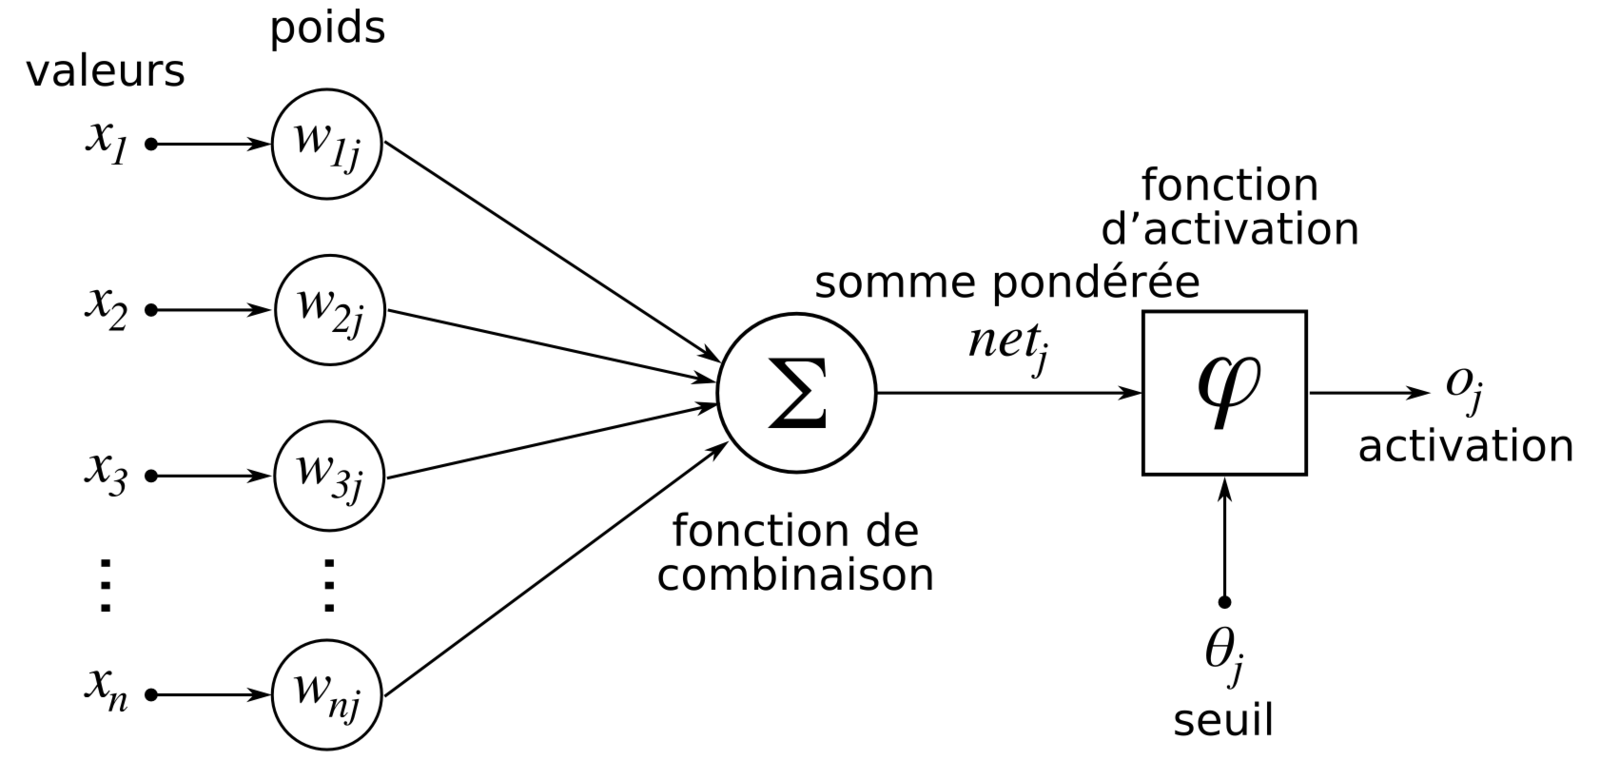
\includegraphics[width=.75\linewidth]{images/neurone}
		\caption{Neurone détaillé}
	\end{figure}
	
	Chaque neurone prend une valeur entre 0 et 1, déterminée par ce qu'il reçoit en entrée et par une fonction d'activation. On voit, à gauche de l'image, des valeurs $x_1, x_2,x x_3, ..., x_n$. Ce sont les valeurs déduites de la couche précédente. Les poids, notés ici $w$ représentent l'impact qu'ont ces valeurs sur le neurone. Vient ensuite la fonction d'activation. Son rôle est "d'écraser" la valeur de la somme pondérée ($\sum_{k=0}^{N}x_kw_{k}$) pour qu'elle appartienne à un intervalle voulu. On la notera $\varphi$.\\
	
	Avant de commencer la partie mathématique, voici un récapitulatif des indices et exposants utilisés dans les équations ci-dessous :
	$$
	\begin{cases}
		L : \text{numéro de couche, la couche d'entrée est $L = 1$}\\
		k : \text{numéro du neurone de la couche d'entrée}\\
		K : \text{nombre de neurones de la couche d'entrée (si on ne compte pas le biais noté $x_0$)}\\
		n : \text{numéro du neurone de la couche $L$}\\
		N : \text{nombre de neurones de la couche $L$ (si on ne compte pas le biais noté $a_0^{(L)}$)}\\
		m : \text{numéro du neurone de la couche $L-1$}\\
		M : \text{nombre de neurones de la couche $L-1$ (si on ne compte pas le biais noté $a_0^{(L-1)}$)}
	\end{cases}
	$$
	
	On peut donc écrire que la valeur du premier neurone de la première couche cachée est : 
	$$a_1^{(2)} = \varphi\left(\sum_{k=0}^{K}x_kw_{k1}^{(1)}\right)$$
	On peut le généraliser au $n^{\text{ème}}$ neurone de cette couche :
	$$a_n^{(2)} = \varphi\left(\sum_{k=0}^{K}x_kw_{kn}^{(1)}\right)$$
	
	\noindent Si l'on passe à la couche suivante, le premier neurone celle-ci s'écrit comme la somme pondérée des valeurs des neurones de la couche précédentes multipliées par leur poids sur ce neurone : 
	$$a_1^{(3)}  = \varphi\left(\sum_{i=0}^{N}a_i^{(2)}w_{i1}^{(2)}\right)$$
	C'est donc une somme de sommes et pour le $n^{\text{ème}}$ neurone de la 2\ieme{} couche cachée, elle vaut :
	$$a_n^{(3)} = \varphi\left(\sum_{i=0}^{N}\varphi\left(\sum_{k=0}^{K}x_kw_{kn}^{(1)}\right)a_i w_{i1}^{(2)}\right)$$
	
	\noindent Finalement, pour n'importe quel neurone,on a :
	$$ a_n^{(L)} = \varphi\left(\sum_{m=0}^{M}\left[...\left[\varphi\left(\sum_{i=0}^{N}\varPhi\left(\sum_{k=0}^{K}x_kw_{kn}^{(1)}\right)w_{in}^{(2)}\right)\right]...\right]w_{nm}^{(L)}\right) $$
	
	
\subsection{Fonction d'activation}
	Nous n'avons pas encore parler de la fonction d'activation, ici $\varphi$. Son rôle est de dire si un neurone doit être "actif" ou non, selon la valeur de la somme pondérée. Nous nous attarderons pas trop dessus mais il faut tout de même savoir quelle fonction prendre on utilise afin de la dériver par la suite. Une des fonctions d'activation les plus répandues est la fonction sigmoïde définie par $\sigma(x) = \frac{e^x}{1+e^x}$.
	
\subsection{Fonction erreur}
	Après la chaque phase avant, on obtient des valeurs pour chacun des neurones de la couche de sortie. Cependant ces valeurs ont été calculées à partir d'entrées initialisées aléatoirement. Il faut donc comparer ces résultats avec ceux attendus. 

	
	
\section{Application des algorithmes}